% \usepackage[hyphens,spaces,obeyspaces]{url}
% \usepackage{algorithm}
% \usepackage{algorithmic}
% \usepackage[dvips]{graphicx}
% \usepackage{latexsym}
% \usepackage{color}
% \usepackage{amsmath}
% \usepackage{amssymb}
% \usepackage{amsfonts}
% \usepackage{enumerate}
% \usepackage{bm}
% \usepackage{cases}
% \usepackage{latexsym}
% \usepackage{comment}
% \usepackage{listings}
% \usepackage{longtable}
% \usepackage{nogamacro}
% \usepackage{multirow}
% \usepackage{float}

%-----------------------CUSTOM COMMAND-------------------------------
% paper title
% Titles are generally capitalized except for words such as a, an, and, as,
% at, but, by, for, in, nor, of, on, or, the, to and up, which are usually
% not capitalized unless they are the first or last word of the title.
% Linebreaks \\ can be used within to get better formatting as desired.
% Do not put math or special symbols in the title.
\title{A Comparative Implementation of GLV Technique on KSS-16 Curve}

Pairing-based protocols are getting popular in many cryptographic applications. 
Pairing algorithms involve computations on elements in all three pairing groups, $\mathbb{G}_1$, $\mathbb{G}_2$ and $\mathbb{G}_3$; however, most protocols usually require additional scalar multiplication and exponentiation in any of these three groups. 
The Gallant-Lambert-Vanstone (GLV) method is an elegant technique to accelerate the scalar multiplication which can reduce the number of elliptic curve doubling by using Straus-Shamir simultaneous multi-scalar multiplication technique.
However, efficiently computable endomorphisms are required to apply GLV for the elliptic curves. 
This paper shows the GLV technique by deriving efficiently computable endomorphism for Kachisa-Schaefer-Scott (KSS) curve defined over degree 16 extension field.
In addition, the authors show explicit formulas to compute the GLV method together with Straus-Shamir simultaneous multi-scalar multiplication technique for 2, 4 and 8 dimensions in $\g2$ group. 
The comparative implementation shows that dimension 4 gives faster computational time than dimension 8 and 2. 

\section{Introduction}
% The authors in \cite{self_indo17}  that KSS-16 is a better alternative for Optimal-Ate pairing than widely studied BN curve.

The independent works of  Sakai et al. \cite{sakai2000cryptosystems} and Joux et al. \cite{joux} set up a new type of public key cryptography based on bilinear pairing over the elliptic curve.
Since then it has encouraged to invent several innovative pairing-based cryptographic applications such as Boneh et al.'s short signature \cite{shortsign} and short group signature authentication \cite{group_sign_1}, those have increased the popularity of pairing-based cryptographic research.
However, most pairing-based protocols require additional scalar multiplication (SCM) or exponentiation in the pairing groups beside the pairing.
Moreover, some protocols \cite{groth2010short} require only a single pairing and several scalar multiplications. 
Therefore, we are interested in such peripheral operation that is the scalar multiplication of pairing-based protocols.

In general, pairing is a bilinear map of two rational point groups $\G1$ and $\g2$ to a multiplicative group $\g3$ \cite{Silverman}.
The typical notation of pairing is $\G1 \times \g2 \rightarrow \g3$.
% In  Ate-based pairing, $\G1$, $\g2$ and $\g3$ are defined as:
% \begin{eqnarray}\label{eq:g_1}
% \G1 & = &  E(\F{p}{k}) [r] \cap \text{Ker}(\pi_p - [1]), \nonumber \\
% \g2 & = &  E(\F{p}{k}) [r] \cap \text{Ker}(\pi_p - [p]), \nonumber \\
% \g3 & = & \mF{p}{k}/(\mF{p}{k})^r, \nonumber
% \end{eqnarray}
% \begin{equation}
% \alpha : \G1 \times \g2 \rightarrow \g3,  \nonumber
% \end{equation}
% where $\alpha$ denotes Ate pairing.
Pairings are often defined over a certain extension field $\FPK$, where $p$ is the prime number, also known as characteristics  and $k$  is the minimum extension degree for pairing also called \textit{embedding} degree. 
More importantly, pairing is performed over the special form of elliptic curves typically known as pairing-friendly curves.
There are several widely studied pairing-friendly curve families i.e. Barreto-Naehrig (BN), Barreto-Lynn-Scott (BLS) curves\cite{taxonomy}. 
The set of rational points $E(\FPK)$ are defined over a certain pairing-friendly curve of embedded extension field of degree $k$.
This paper has considered Kachisa-Schaefer-Scott (KSS) \cite{kss} pairing-friendly curves of embedding degree $k=16$ (KSS-16) in the context of Optimal-ate pairing.
The motivation to work on KSS-16 curve came from the recent work of Barbulescu et al. \cite{sylvain_new_param} and Khandaker et al. \cite{self_indo17}, where they concluded that with the recent parameters for pairing-based protocols, KSS-16 curve is a better choice for Optimal-ate pairing over BN curve.

Scalar multiplication dominates the execution time of any elliptic curve cryptography (ECC) algorithms.
The common approach to accelerate scalar multiplication are log-step algorithm such as binary and non-adjacent form (NAF) methods.
However, in the context of asymmetric pairing where there exists no efficiently computable isomorphism between $\G1$ and $\g2$, more efficient approach is to use GLV \cite{sakemi_skew, khandaker2017improvement}.
In order to accelerate scalar multiplication, Gallant-Lambert-Vanstone \cite{gallant2001faster} proposed a technique for rational points of prime order known as GLV method.
Fundamentally, it divides the scalar into half of the bit length of the original one that reduces the number of doubling.
The critical point of this technique is, there should have to be an efficiently computable endomorphism. 
Otherwise, the advantage obtained from reduced doubling will have no effect on the acceleration. 


There is a vast literature on GLV decomposition in pairing-friendly curves i.e.  Barreto-Naehrig \cite{BN}, Kachisa-Schaefer-Scott (KSS) curve of embedding degree 18,  \cite{sakemi_skew, khandaker2017improvement, nogami_scm_ate, faz2015efficient, galbraith2011endomorphisms}. 
The common fact of in such literature is, they all applied GLV on sextic twisted curves. 
However, in our knowledge till date, there is no literature on GLV decomposition for  KSS curve of embedding degree 16 where at most degree 4 twist is available.

The major contributions of this paper are (\RNum{1}) obtaining the endomorphism to enable GLV decomposition for $\g2$ rational point in KSS-16 curve. 
(\RNum{2}) Deriving the dimension 2, 4 and 8 GLV decomposition along with finding efficiently computable Frobenius maps. (\RNum{3}) Implementation of the derived techniques and their comparison. 
This paper shows that increasing the dimension of decomposition not necessarily accelerate the scalar multiplication. 
In the case of $\g2$ points of KSS-16 curve, our experiment finds that dimension 4 is the fastest. 
%On the other hand, dimension 8 is faster than dimension 2 but close to dimension 2 with joint sparse form. 

Throughout this paper, $p$ and $k$ denote characteristic and embedding extension degree respectively. $\F{p}{k}$ denotes $k$-th extension field over prime field $\Fp$ and $\mF{p}{k}$ denotes the multiplicative group in $\F{p}{k}$.

%%-----------------------FUNDAMENTAL-------------------------------------------------------
\section{Fundamentals of Elliptic Curve and Pairing}\label{sec:1}
\subsection{Kachisa-Schaefer-Scott (KSS) Curve \cite{kss}}
Kachisa, Schaefer, and Scott proposed a new family of  parameterized non super-singular pairing-friendly elliptic curves of embedding degree $k = \left\lbrace 16, 18, 32, 36, 40\right\rbrace$.
In this paper, we are interested in the KSS curve whose embedding degree is 16. 
Unlike mostly used degree 6 twist, this curve offers at most degree 4 twist often named as the \textit{quartic twist}.

In what follows, this paper considers  the KSS curve of embedding degree $k =16$, denoted as \textit{KSS-16}, defined over extension field $\FPSN$ as follows:
\begin{equation}\label{eq:KSS_16}
E/\FPSN:y^2=x^3+ax, \quad \mbox{$a \neq 0$},
\end{equation}
where $x,y \in \FPSN$. 
As a typical feature, its properties are parameterized by the polynomial formulas of integer $u$ as follows:
\begin{subequations}
	\begin{eqnarray}
	p(u) &= & (u^{10} +2u^9 +5u^8 +48u^6 +152u^5 +240u^4   \nonumber \\ 
	&& +625u^2 +2398u +3125)/980,  \\\label{eq:kss_16_char}
	r(u) &= & (u^8 +48u^4 +625)/61255, \label{eq:kss_16_degree}  \\
	t(u) &=& (2u^5 +41u+35)/35, \label{eq:kss_16_trace} 
	\end{eqnarray}
\end{subequations} 
where the tuple $(p,r,t)$ are \textit{characteristic}, \textit{group order} and \textit{Frobenius trace} respectively.
The integer  $u$  denotes the pairing parameter conform to the condition $u \equiv 25$ or $45$ (mod $70$). 

\subsection{Point Addition and Doubling}
Let $E(\f{p^k})$ be the set of all rational points on the curve $E$ including the point at infinity $\mathcal{O}$.
$\#E(\f{p^k})$ denotes the total number of point in $E(\f{p^k})$.
Let us consider two rational points using the affine coordinates as $P_1= (x_1, y_1)$, $P_2 = (x_2, y_2)$, and their addition $R = P_1 + P_2$, where $\textit{R} = (x_3, y_3)$ and $P_1, P_2, R \in E(\FPK)$. Then the $x$ and $y$ coordinates of $R$ are calculated as follows:

\begin{subequations}
\begin{eqnarray}\label{eq:point_add}
x_3 & = & \lambda^2-x_1-x_2 ,\\
 y_3 & = &(x_1-x_3)\lambda - y_1, 
\end{eqnarray}
where $\lambda$ is the tangent at the point on the curve given as follows:
\begin{equation}\label{eq:point_solpe}
\textstyle \lambda = 
\begin{cases}
 \textstyle \frac{y_2 - y_1}{ x_2 -x_1}; \quad \mbox{$P_1 \neq P_2$},\\
 \textstyle \frac{3x_1^2+a}{2y_1}; \quad  \mbox{$P_1 = P_2$},\\
\end{cases}
\end{equation}
\end{subequations}
and $\cal O$ is the additive unity in $E(\f{p^k})$. If $P_1 \neq P_2$ then $P_1+P_2$ is called elliptic curve addition (ECA). If $P_1=P_2$ then $P_1+P_2=2P_1$, which is known as elliptic curve doubling (ECD). 

\subsection{Elliptic Curve Scalar Multiplication}
Let scalar $s$ is $0 \leq s < r$, where $r$ is the order of the target rational point group. Scalar multiplication of rational points $P_1$, denoted as $[s]P_1$ is calculated by $(s-1)$-times additions of $P_1$ as,
\begin{equation}\label{scalar_mul}
[s]P_1 = \sum_{i = 0}^{ s-1 } P_1, \quad \text{$0 \leq s < r$}.
\end{equation}
When $s = r$, then $[r]P_1 = \mathcal{O}$, where $r$ is the order of the curve. Let $[s]P_1 = P_2$, and value of $s$ is not obtained, then the solving $s$ from $P_1$ and $P_2$ is known as the elliptic curve discrete logarithm problem (ECDLP). 
The difficulty level of solving ECDLP defines the security strength of elliptic curve cryptography.

\subsection{Extension Field Arithmetic for Pairing}
While implementing pairing-based protocols, a major speedup comes from the efficient finite field implementation.
Therefore, it is common to apply the towering technique to efficiently carry out the extension field operations.
In what follows, the $\FPSN$ extension field is constructed using the following towering with help of the irreducible binomials given in \eqref{towering_1}.
For such construction, in addition with $4|p-1$, $p$ satisfies $p \equiv 3, 5 \bmod 8$.  
\begin{equation}\label{towering_1}
\begin{cases}
\F{p}{2} = \F{p}{}[\alpha]/(\alpha^2-c),  \\ 
\F{p}{4} = \F{p}{2}[\beta]/(\beta^2-\alpha),  \\ 
\F{p}{8} = \F{p}{4}[\gamma]/(\gamma^2-\beta), \\ 
\F{p}{16} = \F{p}{8}[\omega]/(\omega^2-\gamma), \\ 
\end{cases}
\end{equation}
where  $c$ is a quadratic non-residue  ($\QNR$) in $\Fp$. 
This paper considers  $c = 2$ , where $X^{16}-2$ is irreducible in $\FPSN$.

\subsection{Extension Field Arithmetic of $\FPSN$}
% For any platform, multiplication, squaring and inversion are regarded as computationally expensive than addition or subtraction. 
%For convenient estimation of the total pairing cost, we count operations in $\Fp$ for extension field arithmetic.
Towering allows to efficiently carry out multiplication and squaring operation in the extension fields.
\tbref{tab_fpoperation} shows operation count for Karatsuba based multiplication and Devegili et al.'s \cite{devegili2006multiplication} complex squaring technique for squaring. 
\renewcommand{\baselinestretch}{1.5}
\begin{table}[t]
\caption{Number of arithmetic operations in  $\FPSN$ based on Type-I towering \eqref{towering_1}.}
\label{tab_fpoperation}
	%\caption{Number of arithmetic operations in  $\FPSN$ based on Type-I towering \eqref{towering_1}.}
	\centering
	\resizebox{\columnwidth}{!}{
		\begin{tabular}{|l|l|}
			\hline 
			Multiplication & Squaring \\
			\hline 
			$M_{2} = 3M_p + 5A_p+1m_\alpha \rightarrow 3M_p $ &  $S_{2} = 2M_p+6A_p+ \rightarrow 2M_p $\\ 
			$M_{4} = 2M_{2}+5A_{2}+1m_\beta \rightarrow 9M_p $ &  $S_{4} = 2M_{2}+5A_{2}+2m_\beta \rightarrow 6M_p $\\ 
			$M_{8} = 3M_{4}+5A_{4}+1m_\gamma \rightarrow 27M_p $ &  $S_{8} = 2M_{4}+5A_{4}+2m_\gamma \rightarrow 18M_p $\\ 
			$M_{{16}} = 3M_{8}+5A_{8}+1m_\omega \rightarrow 81M_p $ &  $S_{{16}} = 2M_{8}+5A_{8}+2m_\omega \rightarrow 54M_p $\\ 
			\hline 
		\end{tabular} }
\end{table}
\renewcommand{\baselinestretch}{1.0}
The arithmetic operations in $\Fp$ are denoted as $M_p$ for a multiplication, $S_p$ for a squaring, $I_p$ for an inversion.
The $m$ with Greek alphabet and $M$ with numeric suffix denote multiplication with basis element and multiplication in extension field respectively.
Since, $c=2$ in \eqref{towering_1}, therefore, the multiplication by the basis element $\alpha$ is carried out by 1 addition in $\Fp$.

\subsection{Optimal-Ate Pairing on KSS-16 Curve}
In the context of pairing on the KSS-16 curves, the valid bilinear map $e:\G1 \times \g2 \rightarrow \g3$ takes input from two additive rational point groups $\G1, \g2$ 
and output an element in the multiplicative group $\g3$ of order $r$. 
$\G1$, $\g2$ and $\g3$ are defined as follows:
\begin{eqnarray}\label{eq:g1}
\G1 & = &  E(\FP) [r] \cap \text{Ker}(\pi_p - [1]), \nonumber \\
\g2 & = &  E(\F{p}{k}) [r] \cap \text{Ker}(\pi_p - [p]), \nonumber \\
\g3 & = & \mF{p}{k}/(\mF{p}{k})^r, \nonumber
\end{eqnarray}
where $E(\F{p}{k})[r]$ denotes rational points of order $r$ and $[n]$ is scalar multiplication for a rational point. 
Let $\pi_p$ denotes the Frobenius endomorphism given as $\pi_p: (x,y) \mapsto (x^p,y^p)$.

Unless otherwise stated, the rest of the paper considers $P \in \G1 \subset E(\FP)$ and  $Q \in \g2 \subset  E(\FPSN)$, where, $Q$ satisfies $[\pi_p -p]Q = \cal O$.
The map $e$ involves two major steps named Miller's loop followed by the final exponentiation.
%The optimal-ate pairing \cite{op_ate_p} proposed by Vercauteren reduces the Miller's loop length  to $\lfloor \log_2 u \rfloor = \frac{\lfloor \log_2 r \rfloor }{\varphi(k)} $, where $\varphi$ is the Euler's totient function.
%The choice of the parameter $u$ is an important factor for efficient Miller's algorithm since the smaller hamming weight of $u$ adds advantage by reducing elliptic curve doubling (ECD) inside the loop.
The Optimal-ate pairing \cite{op_ate_p} on KSS-16 elliptic curve is given by Zhang et al. \cite{zhang_L12} and presented by the following map.
\begin{align}
 & e_{opt}: \G1\times \g2 \rightarrow  \g3, \\
&  (P,Q) \longmapsto \left(( f_{u,Q}(P)l_{[u]Q,[p]Q}(P))^{3}l_{Q,Q}(P)\right)^{\frac{{16}-1}{r}}.
\end{align}
The rational function $f_{u,Q}(P)$, line evaluation $l_{[u]Q,[p]Q}$ have computed thanks to the Miller algorithm. 
Then, we have the second step which is the computation of the exponent $\frac{{16}-1}{r}$ named the final exponentiation.

\subsection{Gallant, Lambert, and Vanstone (GLV) Decomposition}
In CRYPTO 2001 \cite{gallant2001faster}, Gallant, Lambert, and Vanstone found that any multiple $[s]Q$ of a point $Q$ of prime order $r$ lying on an elliptic curve with a low-degree endomorphism $\Phi$ over $\FP$ can be calculated as follows:
\begin{equation}
    [s]Q = s_1 Q + s_2 \Phi(Q),  
\end{equation}
where $max{|s_1|,|s_2|}  ~\leq C_1 \sqrt{r}$ for some explicit constant $C_1 > 0$.
The main idea of the GLV trick is it exists essentially in an algorithm that finds a decomposition of an arbitrary scalar multiplication $[s]$ for $s \in  [1,r]$ into two scalar multiplications, while the new scalars having only about half the bit length of the original scalar.
This immediately enables the elimination of half the doubling by employing the Straus-Shamir simultaneous multi-scalar point multiplication. 
Later on Galbraith-Lin-Scott (GLS) have shown that over $\FPT$. 
This paper focuses on such a trick for the KSS-16 curve in the context of Optimal-ate pairing. 

%%---------------------------------------------------PROPOSAL----------------
\section{GLV technique for $\g2$ Rational Point on  KSS-16 Curve} \label{Proposal}
As aforementioned, Optimal-ate pairing is computed over a twisted curve. 
Therefore, the following sections will describe the twist property of KSS-16 curve and the procedure to obtain GLV decomposition in the $\g2$ group of a KSS-16 curve.

\subsection{Quartic Twist of KSS-16 Curves} \label{Quartic_twist}
There exists a \textit{twisted curve} with a group of rational points of order $r$ for a KSS-16 curve. 
This isomorphic rational point group includes a twisted isomorphic point of $Q \in \g2 \subset E(\FPK)$, typically denoted as $Q' \in E'(\FPKD)$, where $k$ is the embedding degree and $d$ is the twist degree.  
Since the pairing-friendly KSS-16 \cite{kss} curve has CM discriminant of $D = 1$ and $4|k$; therefore, a quartic twist is available.

Let $\beta$ be a certain quadratic non-residue in $\FPFR$.  The quartic twisted curve $E'$ of KSS-16  curve $E$ defined in \eqref{eq:KSS_16} and  their isomorphic mapping $\psi_4$ are given as follows:
\begin{eqnarray} 
	E'&:&y^2=x^3+ax\beta^{-1},\;\;\;a\in\Fp, \label{twisted_E} \\ 
	\psi_4&:&E'(\FPFR)[r] \longmapsto E(\FPSN)[r]\cap {\rm Ker}(\pi_p-[p]),\nonumber\\
	&& \quad \quad (x,y)\longmapsto (\beta^{1/2}x,\beta^{3/4}y),\label{map1}
\end{eqnarray}
where Ker($\cdot$) denotes the kernel of the mapping and $\pi_p$ denotes Frobenius mapping  for rational point.

%\tbref{tab_Q} shows the vector representation of $Q = (x_{Q},y_Q) = (\beta^{1/2}x_{Q'},\beta^{3/4}y_{Q'}) \in \FPSN$ according to the given towering in \eqref{towering_1}.
%For the above mapping, the vector representation of Q ∈ G2 is Q = (xQ, yQ) = (β1/2xQ′ , β3/4yQ′ ) ∈ E(Fp16 ) according to the given towering in Eq.(5).
For the above mapping, the vector representation of $Q = (x_{Q},y_Q) = (\beta^{1/2}x_{Q'},\beta^{3/4}y_{Q'}) \in \FPSN$ is obtained according to the given towering in \eqref{towering_1}.
Here, $x_{Q'}$ and $y_{Q'}$ are the coordinates of rational point $Q'$ on quartic twisted curve $E'$. 


% \renewcommand{\baselinestretch}{1.5}
% \begin{table*}[t]
% \caption{Vector representation of $Q = (x_Q,y_Q) \in \g2 \subset E(\mathbb{F}_{{16}})$}
% \label{tab_Q}
% \centering
% % \resizebox{2\columnwidth}{!}{
% \begin{tabular}{|*{17}{c|}}
% \hline 
%  & 1 & $\alpha$ & $\beta$ & $\alpha \beta$ & $\gamma$ & $\alpha \gamma$ & $\beta \gamma$ & $\alpha \beta \gamma$ & $\omega$ & $\alpha \omega$ & $ \beta \omega$ & $\alpha \beta \omega$ & $\gamma \omega$ & $\alpha \gamma \omega$ &$ \beta \gamma \omega$ & $\alpha \beta \gamma \omega$\\
%   \hline 
% $x_Q$ & 0 & 0 & 0 & 0 & $b_4$ & $b_5$ &$ b_6$ & $b_7$ & 0 & 0 & 0 & 0 & 0 & 0 & 0& 0\\
%  \hline 
% $y_Q$ & 0 & 0 & 0 & 0 & 0 & 0 & 0 & 0 & 0 & 0 & 0 & 0 & $b_{12}$ & $b_{13}$ & $b_{14}$ & $b_{15}$\\
% \hline 
% \end{tabular}
% % }
% \end{table*}
% \renewcommand{\baselinestretch}{1.0}

\subsection{Elliptic Curve Operation in Twisted Curve $E'$}
 Since $E'$ in \eqref{twisted_E} is different from $E$, therefore, the elliptic curve addition and doubling operation slightly changed.
Let us consider  $T=(\gamma x_{T'},\gamma \omega y_{T'})$, $Q=(\gamma x_{Q'}, \gamma \omega y_{Q'})$  and  $P=(x_P,y_P) $, where $x_p, y_p \in \Fp$ given in affine coordinates on the curve $E(\FPSN)$ such that $T'=(x_{T'},y_{T'})$, $Q'=(x_{Q'},y_{Q'})$ are in the twisted curve $E'$ defined over $\FPFR$.
Let the elliptic curve doubling of $T+T = R(x_R, y_R)$. 
% The 7-sparse multiplication for KSS-16 can be derived as follows.
%\begin{alignat}
\begin{alignat}{3}
 \lambda & =  \frac{ 3x_{T'}^2 \gamma^2+a}{2 y_{T'} \gamma \omega} = \frac{ 3x_{T'}^2 \gamma \omega^{-1}+a (\gamma \omega)^{-1} }{2 y_{T'}}, \nonumber \\
 & = \frac{ (3x_{T'}^2 +a c^{-1} \alpha\beta)\omega}{2 y_{T'}} = \lambda' \omega, \nonumber 
 \end{alignat}
since  $\gamma \omega^{-1} = \omega, (\gamma \omega)^{-1} = \omega \beta^{-1}$, and $a \beta^{-1} = (a + 0\alpha + 0 \beta + 0 \alpha \beta) \beta ^{-1}=a \beta^{-1} = ac^{-1} \alpha \beta$, where $\alpha^2=c$.
Now the ECD are obtained as follows:
\begin{eqnarray}
 x_R &=& (\lambda')^2 \omega^2 \ - 2x_{T'}\gamma   = ((\lambda')^2  \ - 2x_{T'})\gamma, \nonumber \\
 y_R &=& (x_{T'}\lambda' -x_{2T'}\lambda'-y_{T'})\gamma \omega \nonumber.
\end{eqnarray}

The elliptic curve addition phase (i.e. $T\neq Q$) can be written as $T+Q = R(x_R, y_R)$.
\begin{eqnarray}
\lambda &=& \frac{( y_{Q'}-y_{T'})\gamma \omega}{( x_{Q'}-x_{T'})\gamma} = \frac{( y_{Q'}-y_{T'}) \omega}{x_{Q'}-x_{T'}} = \lambda' \omega, \nonumber\\
x_{R} & = & ((\lambda')^2  \ - x_{T'} -x_{Q'})\gamma, \nonumber \\
 y_{R} & = &  (x_{T'}\lambda' -x_{R'}\lambda'-y_{T'})\gamma \omega \nonumber.
\end{eqnarray}
%-------
\subsection{Finding  Endomorphism between $p$ and $u$}
Let us find an endomorphism between the prime $p$ and the integer $u$ from using the Hasse's theorem
\begin{eqnarray}
p+1 - t \equiv 0 \bmod r, \nonumber
\end{eqnarray}
as follows:
\begin{eqnarray}
p & \equiv & t-1 \bmod r, \nonumber \\
35p   & \equiv &  2u^5+41u \bmod r. \label{eq_pt1}
\end{eqnarray}
The modulus of order $r$ defined in \eqref{eq:kss_16_degree} can be expressed as 
\begin{equation}
u^8+48u^4+625 \bmod r \equiv  0 .\label{eq_order_mod}
\end{equation}
From the above equation we approach to find the relation between $p$ and $u$ as follows:
\begin{eqnarray}
2u^8+ 96u^4 + 2 \cdot 5^4\bmod r & \equiv & 0, \nonumber \\
35pu^3-41u^4 + 96u^4 + 2 \cdot 5^4 \bmod r & \equiv & 0,\nonumber \\
35pu^3+55u^4+2\cdot5^4 \bmod r & \equiv & 0, \nonumber \\
7pu^3+11u^4+2\cdot5^3 \bmod r & \equiv & 0, \nonumber \\
11u^4+2\cdot5^3 \bmod r & \equiv & -7pu^3, \nonumber \\
11u+2\cdot5^3u^{-3} \bmod r & \equiv & -7p. \label{eq_p_u_1}
\end{eqnarray}
Let us take 4-th power of both side of the \eqref{eq_p_u_1}.
\begin{alignat}{3}
7^4p^4 &  \equiv (11u+2\cdot5^3u^{-3})^4 \bmod r, \nonumber \\
 %&\equiv & 11^4u^4+4\cdot11^3u^{-3}\cdot2\cdot5^3u^{-3}  \nonumber \\
% & & +  6\cdot11^2u^2\cdot4\cdot5^6u^{-6} + 4 \cdot 11u\cdot2^3\cdot5^9\cdotu^{-9} \nonumber \\
% & & + 2^4\cdot 5^{12}u^{-12} \bmod r\nonumber  \\
 & \equiv  11^4u^4 + 8 \cdot 5^3 11^3 + 24\cdot  5^6 11^2 u^{-4} + 32 \cdot 11 \cdot 5^9u^{-8} \nonumber \\
 &  \quad  + 2^4 5^{12}u^{-12} \bmod r. \label{eq_74p4}
\end{alignat}
Multiplying $u^{-12}$ with \eqref{eq_order_mod} result in the following relation.
\begin{equation}
    u^{-4}+48u^{-8}+5^4u^{-12} \bmod r  \equiv   0 \nonumber. \\
\end{equation}
Afterward multiplying $2^4 5^{8}$ with the above equation is obtained as follows:
\begin{equation}
    2^4 5^{8}u^{-4}+ 48 \cdot  2^4 5^{8}u^{-8}+  2^4 5^{12} u^{-12} \bmod r \equiv   0 \nonumber,
\end{equation}
which helps to simplify the \eqref{eq_74p4} as 
%\begin{eqnarray}
% 7^4p^4 &\equiv & 11^4u^4 + 8\cdot 5^3 11^3 + 5^6 11^2 24 u^{-4} +  32 \cdot 5^9 11u^{-8} \nonumber \\
% & &   - 2^4  5^{8}u^{-4} - 2^4 48 \cdot 5^{8}u^{-8}\bmod r, \nonumber \\
% & \equiv & 11^4u^4+ 8 \cdot 5^3  11^3+2504 \cdot 5^6u^{-4}  \nonumber \\
% && +  5^8 992u^{-8} \bmod r. \label{eq_74p4_2}
%\end{eqnarray}
\begin{alignat}{2}
7^4p^4 &\equiv  11^4u^4 + 8\cdot 5^3 11^3 + 24 \cdot 5^6 11^2 u^{-4} +  32 \cdot 11 \cdot 5^9 u^{-8} \nonumber \\
& \quad   - 2^4  5^{8}u^{-4} - 48 \cdot 2^4 5^{8}u^{-8}\bmod r, \nonumber \\
& \equiv 11^4u^4+ 8 \cdot 5^3  11^3+2504 \cdot 5^6u^{-4}  \nonumber \\
& \quad + 992 \cdot 5^8 u^{-8} \bmod r. \label{eq_74p4_2}
\end{alignat}
At this point let us multiply $992 \cdot 5^4u^{-8}$  with \eqref{eq_order_mod} to obtain
\begin{equation}
     992 \cdot 5^4 +  992 \cdot 48 \cdot  5^4 u^{-4}+ 992 \cdot 5^8u^{-8} \bmod r  \equiv   0. \nonumber
\end{equation}
Using the above relation, \eqref{eq_74p4_2} can be expressed as  
\begin{alignat}{3}
 7^4p^4 & \equiv  11^4u^4+ 8 \cdot 5^311^3+2504 \cdot 5^6u^{-4} - 992 \cdot48 \cdot 5^4 u^{-4}  \nonumber \\
 & \quad -992 \cdot 5^4 \bmod r,  \nonumber \\
 & \equiv  11^4x^4+5688 \cdot 5^3 +14984 \cdot 5^4 u^{-4} \bmod r. \label{eq_74p4_3} 
\end{alignat}
Now, let us multiply $14984u^{-4}$ with \eqref{eq_order_mod} to obtain the following equation as
\begin{equation}
    14984u^4+14984 \cdot 48+ 14984 \cdot 5^4 \bmod r \equiv 0.
\end{equation}
Substituting the above equation in \eqref{eq_74p4_3} the final relation can be obtained as follows:
%\begin{eqnarray}
\begin{alignat}{3}
 7^4p^4  & \equiv 11^4x^4 + 5688 \cdot 5^3 - 14984 u^{4} - 14984 \cdot 48 \bmod r, \nonumber \\
  &\equiv  (14641-14984)u^4 + (711000-719232) \bmod r, \nonumber \\
  & \equiv  -343 u^4 -8232 \bmod r, \nonumber \\
  7p^4 & \equiv  -u^4 -24 \bmod r.  \label{eq_p_u_relation}
%\end{eqnarray}
\end{alignat}
Finally, $u^4 \equiv -7p^4-24 \bmod r$ is the endomorphism we are interested in.
Since the relation is obtained for $u^4$, therefore, we can apply it for 2 dimension GLV decomposition.
The reason can be anticipated clearly as the order $r$ is a polynomial of degree 8 of the integer $u$.

\subsection{GLV for the Group Having Order $r(u)$}
We can apply at most $\varphi(16)= 8$ dimension GLV decomposition for $\g2$ rational point group; since the KSS-16 is a curve defined over an extension field of degree 16.
Here $\varphi$ is the Euler's totient function.
However, as discussed in the introduction, there is always a trade-off between the number of pre-computation and the dimension of GLV for any curve. 

In the context of KSS-16, $p^{16}-1$ can be divisible by $r$ from the definition of pairing.  Therefore, we got the following equations.
\begin{subequations}
\begin{alignat}{3}
p^{16} &\equiv 1~(\bmod~r), \\
\label{p8_m1}
p^{8}&\equiv -1~(\bmod~r),\\
\label{p4_i}
p^{4} &\equiv \sqrt{-1} \equiv i~(\bmod~r).
\end{alignat}
\end{subequations}
Since $-1$ is a QNR in $\FP$, therefore, $\sqrt{-1}$ exists in $\Fp$. 
\subsubsection{Dimension 8 GLV decomposition}
Since order $r$ of  the KSS-16 curve defined in \eqref{eq:kss_16_degree} is a degree 8 polynomial of integer $u$, therefore, to obtain dimension 8 GLV decomposition of a scalar $s$ as the following form
\begin{equation}
 s = s_0 + u s_1 + u^2 s_2 + u^3 s_3 + u^4 s_4 + u^5 s_5 + u^6 s_6 + u^7 s_7, \nonumber
\end{equation}
we need to find a relation between above degrees of $u$ and prime $p$. 
Let us first obtain a relation between degree 1 of $u$ and $p$ as follows:
\begin{alignat}{3}
p &\equiv t-1~(\bmod~r), \nonumber \\
35p &\equiv 2u^5+41u~(\bmod~r), ~~(\text{see~Eq.}(\ref{eq_pt1}))\nonumber \\
35p &\equiv u(2u^4+41)~(\bmod~r), \nonumber \\
35p &\equiv u(2(-7p^4-24)+41)~(\bmod~r), ~~(\text{see~Eq.}(\ref{eq_p_u_relation})) \nonumber \\
35p &\equiv u(-14p^4-7)~(\bmod~r), \nonumber \\
5p &\equiv u(-2p^4-1)~(\bmod~r), \nonumber \\
u &\equiv 5p(-2p^4-1)^{-1}~(\bmod~r), \nonumber \\
u &\equiv 5p(-2i-1)^{-1}~(\bmod~r), ~~(\text{see~Eq.}(\ref{p4_i})) \nonumber \\
u &\equiv 5p(-2i-1)^{-1}(-2i-1)(2i-1)/5~(\bmod~r), \nonumber \\
u &\equiv p(2i-1)~(\bmod~r), \nonumber \\
u &\equiv 2p^5-p~(\bmod~r). \label{equ} 
\end{alignat}

\subsubsection{Dimension 4 GLV decomposition}
To obtain the dimension 4 decomposition, we derive the relation between degree 2 of $u$ and $p$ as follows:
\begin {alignat}{3}
u^2 &\equiv p^2(2p^4-1)^2~(\bmod~r), \nonumber \\
%u^2 &\equiv p^2(4p^8-4p^4+1)~(\bmod~r), \nonumber \\
u^2 &\equiv p^2(-4-4p^4+1)~(\bmod~r),  ~~(\text{see~Eq.}(\ref{p8_m1})) \nonumber \\
%u^2 &\equiv p^2(-4p^4-3)~(\bmod~r), \nonumber \\
u^2 &\equiv -4p^6-3p^2~(\bmod~r). \label{equ2}
\end{alignat}


\subsubsection{Dimension 2 GLV decomposition}
 Modular equation for dimension 2 GLV is already obtained in \eqref{eq_p_u_relation}.
However, we can verify that as follows:
\begin{alignat}{3}
u^4 &\equiv p^4(-4p^4-3)^2~(\bmod~r), \nonumber \\
%u^4 &\equiv p^4(16p^8+24p^4+9)~(\bmod~r), \nonumber \\
u^4 &\equiv p^4(-16+24p^4+9)~(\bmod~r),  ~~(\text{see~Eq.}(\ref{p8_m1})) \nonumber \\
%u^4 &\equiv p^4(24p^4-7)~(\bmod~r),\nonumber \\
%u^4 &\equiv 24p^8-7p^4~(\bmod~r), \nonumber \\
u^4 &\equiv -7p^4-24~(\bmod~r). ~~(\text{see~Eq.}(\ref{p8_m1})) \label{equ4}
\end{alignat}

Beside $u, u^2$ and $u^4$ we also need to find the endomorphisms for $u^3, u^5, u^6$ and $u^7$.
Using the above \eqref{equ}, \eqref{equ2} and \eqref{equ4}, they can be given as follows:
\begin{alignat}{3}
 u^3 & \equiv  11p^3-2p^7, \nonumber \\
 u^5 & \equiv 38p -41p^5,\nonumber \\
 u^6 & \equiv  117p^6+44p^2, \nonumber \\
 u^7 & \equiv  -278p^3 -29p^7. \nonumber 
\end{alignat}

\subsubsection{Dimension 2 GLV with Joint Sparse Form}
In \cite{solinas2001JFS}, Solinas proposed a joint sparse form (JSF) for two integers. 
Let say the two integers are $s_0$ and $s_1$. 
The JSF representation of $s_0$ and $s_1$ will ensure that their joint Hamming weight is minimal among all signed binary representations of the same pair of integers. 
Therefore, we combined 2-dimensional GLV with JSF to make the scalar multiplication faster.

\subsection{Applying Straus-Shamir Simultaneous Multi-scalar Multiplication Technique}
In what follows let us denote the 2-dimension as 2-Split, 4-dimension as 4-Split
and 8-dimension as 8-Split scalar multiplication.
In our experimental implementation, we adopted the parameter suggested in \cite{sylvain_new_param}. 
Using \cite{sylvain_new_param}'s settings the integer  $u$ is obtained as $35$-bit and order $r$ as $263$-bit. 
Therefore, the maximum bit length of an $s$ is $\leq 263$-bit.
\subsubsection{2-Split and 4-Split scalar multiplication}
The 2-Split scalar multiplication can be expressed as
\begin{equation}
    [s]Q = [s_0]Q + s_1 [u^4]Q.
\end{equation}
For the above representation, we need at most $2^2$ pre-computed points and 2-bit (one for $s_0$ and another is $s_1$) simultaneous multi-scalar multiplication.
Similarly, 4-Split can be calculated as 
\begin{equation}
    [s]Q = [s_0]Q+s_1[u^2]Q+s_2[u^4]Q+s_3[u^6]Q,
\end{equation}
using $2^4$ pre-computed rational point patterns applied in 4-bit ($s_3,s_2,s_1,s_0$) simultaneous multi-scalar multiplication. 

\subsubsection{8-Split scalar multiplication}
The 8-Split multiplication can be a little bit tricky since the usual way will calculate $2^8$ pre-computed points.
\begin{figure*}
\centering
%\includegraphics[width=1.5\columnwidth]{pre.eps}
	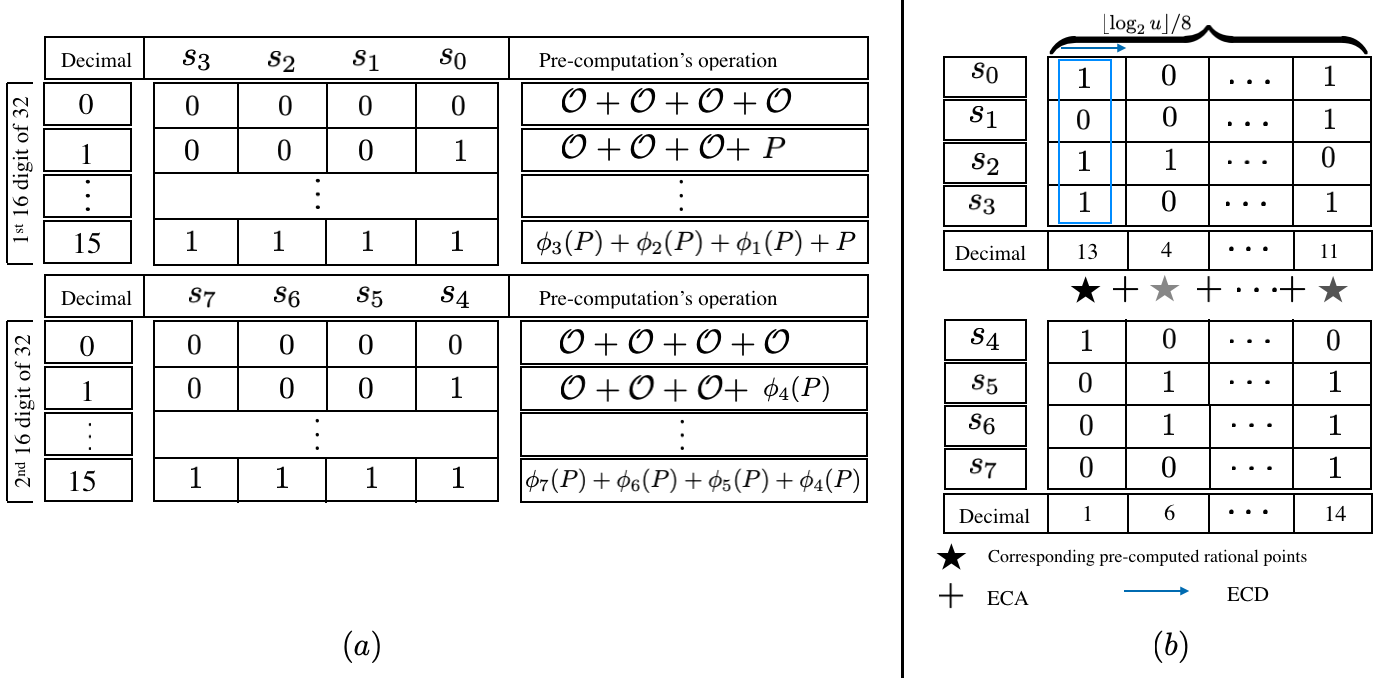
\includegraphics[width=\linewidth,height=.4\textheight, keepaspectratio]{com8split}
\caption{(a) Pre-computation of rational points for dimension 8  GLV. ~ (b) Computation of SCM for dimension 8  GLV.}
\label{precom_figure}
\end{figure*}
 Since $u = 35$-bit,  the maximum length of the scalar after the dimension 8 decomposition will be $\leq 35$-bit.
Therefore, at most 35 pre-computed points will be utilized during the  multi-scalar multiplication.
As a result, we separated the scalar into two groups as $(s_3,s_2,s_1,s_0)$ and $(s_7,s_6,s_5,s_4)$.
Then we pre-computed $2^4 + 2^4 = 32$ rational points.
\fgref{precom_figure}(a) shows the pre-computation steps.  
Among the 32 pre-computed points each of the points will be utilized at least once during multi-scalar multiplication. 
Finally, we combined the result of the two separately  obtained multi-scalar multiplication by one extra elliptic curve addition. 
%\begin{figure}[t]
%\centering
%	\includegraphics[width=\linewidth,height=.4\textheight, keepaspectratio]{com}
%%\includegraphics[scale=0.5]{com.eps}
%\caption{Computation of SCM for dimension 8  GLV.}
%\label{com_figure}
%\end{figure}
As a result we can save $2^8-32 = 224$ pre-computation. 
\fgref{precom_figure}(b) shows the computation of the loop where simultaneous multi-scalar multiplications are carried out. 

To obtain the pre-computed rational points we need to calculate $[p]Q, [p^2]Q, \cdots, [p^7]Q$ as shown in \fgref{precom_figure}(a).
Thanks to Frobenius map which can be calculated with a few multiplications in $\Fp$.
Moreover, since rational points in $\g2$ have isomorphic twisted points in $\g2'\subset E'(\FPFR)$, therefore, skew Frobenius map \cite{sakemi_skew} can be applied as shown in the \secref{sec_tskew_fm}.

\subsection{Skew Frobenius Map to Compute $[p]\bar{Q'}$}
\label{sec_tskew_fm}
From the definition of $Q \in \g2$, we recall that $Q$ satisfies $[\pi_p -p]Q = \cal O$ or $\pi_p(Q) = [p]Q$, which is also applicable for $\bar{Q'}$.
Applying skew Frobenius map we can optimize $[p]\bar{Q'}$ calculation.
The detailed procedure to obtain the skew Frobenius map of $Q' = (x_{Q'}, y_{Q'}) \in \g2' \subset E'(\FPFR)$ is given bellow:
\begin{subequations}
\begin{equation}
(x_{Q'}\gamma )^p  =   (x_{Q'})^p \gamma^p. \nonumber \\
\end{equation}
After remapping 
\begin{eqnarray}
 (x_{Q'})^p \gamma^{p-1} & = &  (x_{Q'})^p (\gamma^2)^{\frac{p-1}{2}}, \nonumber
\end{eqnarray}
 \end{subequations} 
The $(\gamma^2)^{\frac{p-1}{2}} $ term can be simplified as follows:
 \begin{subequations}
 \begin{eqnarray}
 \label{gama1}
(\gamma^2)^{\frac{p-1}{2}} & = & (\beta^2)^{\frac{p-1}{4}}, \mbox{\quad since $p \equiv 5 \bmod 8$,} \nonumber \\
& = & (\alpha)^{\frac{p-1}{4} -1}\alpha, \nonumber \\
& = & (\alpha^2)^{\frac{p-5}{8}}\alpha, \nonumber \\
& = & c^{\frac{p-5}{8}}\alpha.
\end{eqnarray}
Recall that $c=2$ in \eqref{towering_1}. 
% The  $(x_{Q'})^p \in \FPFR$ can be calculated as Frobenius map in $\FPFR$  as 
% \begin{eqnarray}
% x_{Q}^p &=& (a_0+a_1\alpha+a_2\beta+a+3 \alpha\beta)^p \nonumber \\
%  & = & ( -a_1c + a_0 \alpha -a_3c \beta +a_2\alpha \beta) c^{\frac{3p-7}{8}}
% \end{eqnarray} 

Similar way the skew Frobenius map of $y_{Q'}$ is given as,
\begin{equation}\label{skewfm}
(y_{Q'}\gamma \omega )^p  =   (y_{Q'})^p \gamma^p \omega^p. \nonumber \\
\end{equation}
After remapping 
\begin{eqnarray}
 (y_{Q'})^p \gamma^{p-1} \omega^{p-1} & = &  (y_{Q'})^p (\gamma^2)^{\frac{p-1}{2}} (\omega^2)^{\frac{p-1}{2}}. \nonumber
\end{eqnarray}
 $(\gamma^2)^{\frac{p-1}{2}}$ is calculated same as \eqref{gama1}. 
 The $(\omega^2)^{\frac{p-1}{2}}$ term is calculated as follows:
\begin{eqnarray}
(\omega^2)^{\frac{p-1}{2}} & = & (\gamma^2)^{\frac{p-1}{4}},\mbox{\quad since $p \equiv 5 \bmod 8$,}\nonumber \\
& = &  \beta^{\frac{p-1}{4} -1} \beta, \nonumber \\
%& = &  ( \beta^2)^{\frac{p-5}{8}} \beta, \nonumber \\
& = &  ( \alpha)^{\frac{p-5}{8}} \beta, \nonumber \\
& = &  ( \alpha)^{\frac{p-5}{8}-1}  \alpha \beta, \nonumber \\
& = &  ( \alpha^2)^{\frac{p-13}{16}}  \alpha \beta, \nonumber \\
& = &  c^{\frac{p-13}{16}}  \alpha \beta. \nonumber
\end{eqnarray}
 \end{subequations}
 The above constant terms will be pre-calculated.
 Now the $x_{Q'})^p, (y_{Q'})^p \in \FPFR$ can be easily calculated where the coefficients will change positions and sign while multiplying with basis elements. For example  $ (x_{Q'})^p (\gamma^2)^{\frac{p-1}{2}} \in \FPFR$ can be calculated as 
%  The  $(y_{Q'})^p \in \FPFR$ can be calculated as Frobenius map in $\FPFR$ same as 
\begin{eqnarray}
 (x_{Q'})^p (\gamma^2)^{\frac{p-1}{2}} &=& (a_0+a_1\alpha+a_2\beta+a_3 \alpha\beta)^p c^{\frac{p-5}{8}}\alpha, \nonumber \\
 & = & ( -a_1c + a_0 \alpha -a_3c \beta +a_2\alpha \beta) c^{\frac{3p-7}{8}}. \nonumber
\end{eqnarray} 
Here it costs 4 multiplication in $\Fp$.
In the similar way $(y_{Q'})^p (\gamma^2)^{\frac{p-1}{2}} (\omega^2)^{\frac{p-1}{2}}$ can be calculated in costing 4 $M_p$.
Therefore, a single skew Frobenius map will cost 8 multiplications in $\Fp$.

During the pre-computation stage of GLV method we also need to compute $[p^2]Q'$, $[p^3]Q'$, $[p^4]Q'$, $[p^5]Q'$, $[p^6]Q'$, $[p^6]Q'$, and $[p^7]Q'$ skew Frobenius maps. 
The procedure is similar to computing $[p]Q'$.
Interestingly, the coefficients basis positions after the skew Frobenius map is similar for $[p]Q'$ and  $[p^5]Q'$ pair; $[p^3]Q$ and $[p^7]Q'$ pair, $[p^2]Q'$ and $[p^6]Q'$ pair.
Only the constant multiples will be different.  


%%---------------------------------Result Analysis-----------------------------
\section{Experimental Result Analysis}
To determine the advantage of the derived GLV techniques, in one hand we applied the twisted mapping to map rational point $Q \in \g2 \subset E(\F{p}{16})$ to its isomorphic point $Q' \in \g2' \subset E'(\F{p}{4})$. 
After that, we performed the scalar multiplication of $Q'$. Then the resulted points are re-mapped to $\g2$ in $\FPSN$.
On the other hand, we performed scalar multiplication using the GLV techniques derived in \secref{Proposal}.
In the experiment, 100 randomly generated scalars of size $\leq r$ (263-bit) are used to calculate SCM for all the cases.
Average value of execution time presented in the millisecond is considered for comparison.
The source of the experimental implementation can be found in Github \footnote{\footurl}.

In the experiment, KSS-16 curve over $\FPSN$ is obtained as $y^2 = x^3 + 1$ by applying the parameters  of Barbulescu et al. \cite{sylvain_new_param}  for 128-bit security level.
\tbref{environment} shows the experiment environment used for comparative evaluation. 
No optimization is done to execute the program in multithreading.
\renewcommand{\baselinestretch}{1.5}
\begin{table}[t]
\centering
\caption{Curve parameters.}
\begin{tabular}{|l|l|l|l|}
\hline
$u= 35$-bit                 & $p$      & $r$      & $t$      \\ \hline
$2^{35}-2^{32}-2^{18}+2^8+1$ & 339 -bit & 263 -bit & 270 -bit \\ \hline
\end{tabular}
\end{table}
\begin{table}[t]
	\centering
	\fontsize{8pt}{8pt}\selectfont
	\caption{Experimental Implementation Environment.}
	\label{environment}
	\resizebox{\columnwidth}{!}{
		\begin{tabular}{|l|l|l|l|l|}
			\hline
			CPU                                                                          & Memory & Compiler  & OS               & \begin{tabular}[c]{@{}l@{}}Language \&\\ Library\end{tabular} \\ \hline
			\begin{tabular}[c]{@{}l@{}}Intel(R) 2.7 GHz \\Core(TM) i5\end{tabular} & 16GB    & 4.2.1 & \begin{tabular}[c]{@{}l@{}}macOS High \\ Sierra 10.13.6\end{tabular}  &\begin{tabular}[c]{@{}l@{}}C\\GMP v 6.1.0 \cite{gmp}\end{tabular}    \\ \hline
			%	\multicolumn{6}{l}{\textsuperscript{*}\footnotesize{Only single core is used from two cores.}}\\
		\end{tabular}
	}
\end{table}
\begin{table}[t]
\centering
\caption{Maximum length of scalar $s$ after GLV decomposition in different dimensions.}
\label{s_length}
\resizebox{\columnwidth}{!}{
\begin{tabular}{|l|l|l|l|l|l|}
\hline
\multirow{2}{*}{\begin{tabular}[c]{@{}l@{}}Max bit length \\ of $s$ after GLV\end{tabular}} & \begin{tabular}[c]{@{}l@{}}Normal\\  binary\end{tabular} & 2-Split  & 2-Split JSF & 4-Split & 8-Split \\ \cline{2-6} 
                                                                                          & 263-bit                                                  & 139-bit & 139-bit    & 69-bit  & 35-bit  \\ \hline
\end{tabular}
}
\end{table}
\begin{table}[t]
	\centering
	\caption{ECD and ECA cost in $E'(\FPFR)$.}
	\label{ecaecd_fp4}
	\begin{tabular}{|l|l|}
		\hline
		ECD cost in $E'(\FPFR)$           & ECA cost in $E'(\FPFR)$  \\ \hline
		$3 M_4 + 8 A_4 + 1 I_4 + 1 M_p$ & $2 M_4 + 6 A_4 + 1 I_4$ \\ \hline
	\end{tabular}
\end{table}
\renewcommand{\baselinestretch}{1.0}
\tbref{s_length} shows the maximum bit length after applying the GLV technique on a scalar of length $263$-bit.
\tbref{ecaecd_fp4} shows the number of operation required to perform single ECA and ECD in $E'(\FPFR)$.
\tbref{tab_res_time} shows the result with respect to ECA and ECD count and time [ms].
From the results, it is clear that 4-Split is the fastest among the techniques followed by the 8-Split.
It is expected that 8-Split should be faster than the 4-Split since it's loop length is half of the 4-Split.
In other words, 8-Split requires about less than half of 4-Split's ECD during loop execution. 
However, combining two 4-Split for one 8-Split increases the number of ECA.
As a result, the total ECA count in the loop for  8-Split is almost same a 4-Split.
The significant fall back of 8-Split compared to 4-Split comes from its number of pre-computed rational points.
Moreover, the total number of pre-computation also increases the other overhead calculations such as initialization, memory allocation, padding $0$ in MSB of the decomposed scalar smaller than the max length. Which also impacts on the execution time. 
\renewcommand{\baselinestretch
}{1.4}
\begin{table}[t]
\centering
\caption{Comparative result of average execution time in [ms] for scalar multiplication.}
\label{tab_res_time}
\begin{tabular}{l|c|c|c|c|c|}
\cline{2-6}
                                    & \multicolumn{2}{l|}{Pre-computation} & \multicolumn{2}{l|}{\begin{tabular}[c]{@{}l@{}}In SCM\\ Algorithm\end{tabular}} & \multirow{2}{*}{Time {[}ms{]}} \\ \cline{1-5}
\multicolumn{1}{|l|}{Operation}     & \#ECA         & \#ECD         & \#ECA                              & \#ECD                               &                                \\ \hline
\multicolumn{1}{|l|}{Normal binary} & 0            & 0                & 120                                    & 262                         \textbf{}           & 42.81                          \\ \hline
\multicolumn{1}{|l|}{2-Split}       & 5                 	& 6                & 98                                    & 138                                     & 28.48                          \\ \hline
\multicolumn{1}{|l|}{2-Split JSF}   & 8                & 6                & 66                                    & 138                                 & 25.16                          \\ \hline
\multicolumn{1}{|l|}{4-Split}       & 24                  & 20               & 64                                     & 68                                     & 19.09                          \\ \hline
\multicolumn{1}{|l|}{8-Split}       & 52                 & 47               & 67                                     & 34                                     & 21.85                          \\ \hline
\end{tabular}
\end{table}
\renewcommand{\baselinestretch}{1.0}



\section{Conclusion}
This paper shows the detailed formula to apply the GLV decomposition together with Straus-Shamir multi-scalar multiplication technique for efficient $\g2$ scalar multiplication which is a major operation in many pairing-based protocols.
The experimental implementation confirms the correctness of the derived technique.
The comparative implementations show that dimension 4 is faster than 8 and 2. 
There is still scope to make the technique better by optimizing the pre-computation which will reduce the number of ECA and ECD.
As a future work, the authors would like to reduce the pre-computation cost by optimizing Frobenius map calculation together with the application of non-adjacent form (NAF) and evaluate the acceleration in a pairing-based protocol. 

ß


